\section{Múltiples tablas}

En el mundo real, existen miles de registros en una tabla, y un registro puede estar conectado con otra tabla, como en el ejemplo anterior de las personas y los números de celular.

El comando \textit{SELECT, FROM y WHERE} permiten consultar información de dos tablas en una misma sentencia (\textit{Tabla \ref{tab: 32}}):
\begin{lstlisting}
    SELECT nombre, apellidos, ciudad, numero, tipo
    FROM Personas, NumCel
    WHERE Personas.id = NumCel.id_personas
\end{lstlisting}
\begin{table}[H]
    \centering
    \caption{Sentencia usando dos tablas}
    \label{tab: 32}
    \begin{tabular}{|l|l|l|l|l|}
        \hline
        \textbf{nombre} & \textbf{apellidos} & \textbf{ciudad} & \textbf{numero} & \textbf{tipo} \\
        \hline
        John    & Smith     & New York      & 555123456 & móvil \\
        \hline
        John    & Smith     & New York      & 943554545 & casa \\
        \hline
        David   & Williams  & Los Angeles   & 331111111 & móvil \\
        \hline
        David   & Williams  & Los Angeles   & 88112233  & trabajo \\
        \hline
        David   & Williams  & Los Angeles   & 999001133 & emergencia \\
        \hline
    \end{tabular}
\end{table}

Utilizar [nombre de tabla].[llave primaria] y [nombre de tabla].[llave foránea] es recomendable para hacer sentencias con más de una tabla, esto hace que las sentencias sean más fáciles de leer, este mismo formato aplica para consultas de una sola tabla:
\begin{center}
    \textit{SELECT PERSONAS.edad FROM Personas}
\end{center}

El siguiente ejemplo es igual a un \textit{SELECT * FROM Personas, NumCel} y muestra simplemente el uso del formato citado anteriormente:
\begin{lstlisting}
    SELECT Personas.nombre, Personas.apellidos, Personas.ciudad, Personas.edad, NumCel.numero, NumCel.tipo
    FROM Personas, NumCel
    WHERE Personas.id = NumCel.id_personas
\end{lstlisting}



\section{JOIN}

Otra forma de combinar dos tablas en una consulta es por medio del comando \textbf{JOIN}, este comando funciona en base en condiciones, utilizaremos el ejemplo del tema anterior pero con \textit{JOIN}:
\begin{lstlisting}
    SELECT nombre, apellidos, ciudad, numero, tipo
    FROM Personas JOIN NumCel
    ON Personas.id = NumCel.id_personas
\end{lstlisting}

\textit{FROM Personas JOIN NumCel} hace la unión entre ambas tablas y \textit{ON} establece la condición. Este comando tiene el aspecto de la \textit{Figura \ref{fig: 3}}:
\begin{figure}[H]
    \centering
    \caption{Concepto de JOIN}
    \label{fig: 3}
    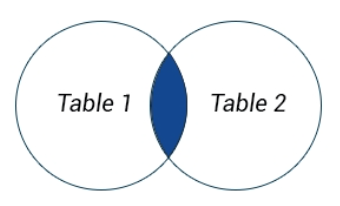
\includegraphics[width=5cm]{ss/join.png}
\end{figure}

Los registros relacionados por la condición de \textit{ON} en ambas tablas aparecen en la zona coloreada.


\subsection{Alias}

En el ejemplo donde recogemos todos los registros de todas las columnas, utilizamos el formato [nombre de tabla].[columna] el cual puede terminar siendo muy largo, es entonces que podemos abreviar el nombre de las columnas a una o pocos caracteres de la siguiente manera:
\begin{lstlisting}
    SELECT P.nombre, P.apellidos, P.ciudad, NC.numero, NC.tipo
    FROM Personas AS P JOIN NumCel AS NC
    ON C.id = NC.id_personas
\end{lstlisting}

Abreviamos el nombre de las tablas en el \textit{SELECT} y definimos esta abreviación con \textit{AS} en el \textit{FROM}, a esto se le llama \textbf{alias de tablas}.


\subsection{Tipos de JOIN}

\textit{JOIN} selecciona los registros que coinciden en ambas tablas, \textbf{LEFT JOIN} selecciona los registros que coinciden en ambas tablas y los de la primer tabla (tabla izquierda), el aspecto de \textit{LEFT JOIN} está en la \textit{Figura \ref{fig: 4}}:
\begin{figure}[H]
    \centering
    \caption{Concepto de LEFT JOIN}
    \label{fig: 4}
    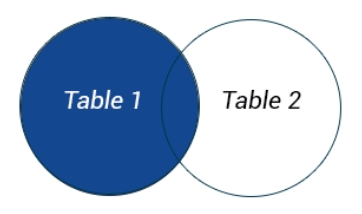
\includegraphics[width=5cm]{ss/left_join.png}
\end{figure}

\textbf{RIGHT JOIN} selecciona los registros que coinciden en ambas tablas y los de la segunda tabla (tabla derecha).



\section{UNION}

Este comando permite combinar los registros de ambas tablas; si en estas tablas hay dos o más registros iguales entre si (duplicados), solo se agrega uno de ellos y no sus duplicados.

Para combinar correctamente los registros, en la sentencia debe haber el mismo número de columnas, tipo de dato y que el orden de las columnas sea el mismo. Para ejemplificar este comando, partiremos la tabla "Personas" en dos y duplicaremos algunos registros, quedando como resultado las siguientes \textit{Tablas}:
\begin{table}[H]
    \centering
    \caption{Tabla "Personas" a la mitad}
    \label{tab: 33}
    \begin{tabular}{|l|l|l|l|l|}
        \hline
        \textbf{id} & \textbf{nombre} & \textbf{apellidos} & \textbf{ciudad} & \textbf{edad} \\
        \hline
        1 & John        & Smith     & New York      & 24 \\
        \hline
        2 & David       & Williams  & Los Angeles   & 42 \\
        \hline
        3 & Chloe       & Anderson  & Chicago       & 65 \\
        \hline
        4 & Emily       & Adams     & Houston       & \textit{NULL} \\
        \hline
        5 & James       & Roberts   & Philadelphia  & 31 \\
        \hline
        6 & John        & Smith     & New York      & 24 \\
        \hline
        7 & David       & Williams  & Los Angeles   & 42 \\
        \hline
    \end{tabular}
\end{table}
\begin{table}[H]
    \centering
    \caption{Tabla "Contactos"}
    \label{tab: 34}
    \begin{tabular}{|l|l|l|l|l|}
        \hline
        \textbf{id} & \textbf{nombre} & \textbf{apellidos} & \textbf{ciudad} & \textbf{edad} \\
        \hline
        1 & Andrew      & Thomas    & New York      & 21 \\
        \hline
        2 & Daniel      & Harris    & New York      & 67 \\
        \hline
        3 & Charlotte   & Walker    & Chicago       & \textit{NULL} \\
        \hline
        4 & Samuel      & Clark     & San Diego     & \textit{NULL} \\
        \hline
        5 & Anthony    & Young     & Los Angeles   & 52 \\
        \hline
        6 & Daniel      & Harris    & New York      & 67 \\
        \hline
        7 & Samuel      & Clark     & San Diego     & \textit{NULL} \\
        \hline
    \end{tabular}
\end{table}

El siguiente ejemplo con \textit{UNION} dará como resultado la \textit{Tabla \ref{tab: 35}}:
\begin{lstlisting}
    SELECT id, nombre, apellidos, ciudad, edad FROM Personas
    UNION
    SELECT id, nombre, apellidos, ciudad, edad FROM Contactos
\end{lstlisting}
\begin{table}[H]
    \centering
    \caption{Unión de las tablas "Personas" y "Contactos"}
    \label{tab: 35}
    \begin{tabular}{|l|l|l|l|l|}
        \hline
        \textbf{id} & \textbf{nombre} & \textbf{apellidos} & \textbf{ciudad} & \textbf{edad} \\
        \hline
        1 & John        & Smith     & New York      & 24 \\
        \hline
        2 & David       & Williams  & Los Angeles   & 42 \\
        \hline
        3 & Chloe       & Anderson  & Chicago       & 65 \\
        \hline
        4 & Emily       & Adams     & Houston       & \textit{NULL} \\
        \hline
        5 & James       & Roberts   & Philadelphia  & 31 \\
        \hline
        6 & Andrew      & Thomas    & New York      & 21 \\
        \hline
        7 & Daniel      & Harris    & New York      & 67 \\
        \hline
        8 & Charlotte   & Walker    & Chicago       & \textit{NULL} \\
        \hline
        9 & Samuel      & Clark     & San Diego     & \textit{NULL} \\
        \hline
        10 & Anthony    & Young     & Los Angeles   & 52 \\
        \hline
    \end{tabular}
\end{table}

Este ejemplo utiliza dos tablas con la misma cantidad de columnas del mismo tipo, muestra todos los registros de ambas tablas menos los registros duplicados. El comando \textbf{UNION ALL} si incluye registros duplicados. En caso de que queramos unir dos tablas, pero alguna de ellas tiene columnas extras que queramos unir, podemos agregar dicha columna en alguna de las sentencias \textit{SELECT}, en el siguiente ejemplo ponemos una columna llamada "trabajo" que solamente existe en la tabla "Contactos" (\textit{Tabla \ref{tab: 36}}):
\begin{lstlisting}
    SELECT id, nombre, apellidos, ciudad, edad, trabajo FROM Contactos
    UNION
    SELECT id, nombre, apellidos, ciudad, edad, NULL FROM Personas
\end{lstlisting}
\begin{table}[H]
    \centering
    \caption{Union de las tablas "Personas" y "Contactos"}
    \label{tab: 36}
    \begin{tabular}{|l|l|l|l|l|l|}
        \hline
        \textbf{id} & \textbf{nombre} & \textbf{apellidos} & \textbf{ciudad} & \textbf{edad} & \textbf{trabajo} \\
        \hline
        1 & John        & Smith     & New York      & 24            & ingeniero \\
        \hline
        2 & David       & Williams  & Los Angeles   & 42            & \textit{NULL} \\
        \hline
        3 & Chloe       & Anderson  & Chicago       & 65            & licenciada \\
        \hline
        4 & Emily       & Adams     & Houston       & \textit{NULL} & \textit{NULL} \\
        \hline
        5 & James       & Roberts   & Philadelphia  & 31            & \textit{NULL} \\
        \hline
        6 & Andrew      & Thomas    & New York      & 21            & \textit{NULL} \\
        \hline
        7 & Daniel      & Harris    & New York      & 67            & ingeniero \\
        \hline
        8 & Charlotte   & Walker    & Chicago       & \textit{NULL} & \textit{NULL} \\
        \hline
        9 & Samuel      & Clark     & San Diego     & \textit{NULL} & \textit{NULL} \\
        \hline
        10 & Anthony    & Young     & Los Angeles   & 52            & licenciado \\
        \hline
    \end{tabular}
\end{table}

Al tener la primer sentencia \textit{SELECT} una columna extra, la segunda debe tener una columna extra para que sean el mismo número de columnas con el mismo tipo de dato, en este caso, asignamos una columna con solamente valores \textit{NULL}.

Podemos utilizar condiciones dentro de las uniones:
\begin{lstlisting}
    SELECT id, nombre, apellidos, ciudad, edad FROM Personas
    WHERE edad > 30
    UNION
    SELECT id, nombre, apellidos, ciudad, edad FROM Contactos
    WHERE edad < 25
\end{lstlisting}
